% !TeX document-id = {beb7ced9-b3cd-42b2-b16a-3ed3c633a1d9}
\documentclass[]             % options: RDPonly, coveronly, nocover
{NASA}                       %   plus standard article class options
%\DeclareRobustCommand{\mmodels}{\mathrel{|}\joinrel\Relbar}

\usepackage[utf8]{inputenc}
\usepackage{csquotes}
\usepackage{setspace}
\usepackage{hyperref}
\usepackage{amsmath, amssymb, amscd, amsthm, amsfonts}
\usepackage{mathtools}
\usepackage{graphicx}
\usepackage{hyperref}
\usepackage{amsthm}
\usepackage[english]{babel}
\usepackage{proof}

\newtheorem{example}{Example}

\newcommand{\B}{\mathbf{B}}
\newcommand{\w}{\mathbf{w}}
\usepackage{proof}
\usepackage{tikz-cd}
\tikzcdset{scale cd/.style={every label/.append style={scale=#1},
    cells={nodes={scale=#1}}}}
\usepackage{stmaryrd}
\hypersetup{
  colorlinks=true,
  linkcolor=blue,
  filecolor=magenta,
  urlcolor=cyan,
  pdftitle={Overleaf Example},
  pdfpagemode=FullScreen,
}
\urlstyle{same}

\newtheorem{theorem}{Theorem}[section]
\newtheorem{corollary}{Corollary}[theorem]
\newtheorem{lemma}[theorem]{Lemma}

\theoremstyle{definition}
\newtheorem{definition}{Definition}[section]

\title{A Survey of Distributed Systems Challenges for Wildland
  Firefighting and Disaster Response}
\author{Lawrence Dunn and Alwyn E. Goodloe}

\AuthorAffiliation{Lawrence Dunn \\ Department of Computer and Information
  Science \\ University of Pennsylvania \\ Philadelphia, PA \\ Alwyn Goodloe\\                                          % for cover page
  NASA Langley Research Center, Hampton, Virginia
}
\NasaCenter{Langley Research Center\\Hampton, Virginia 23681-2199}
\Type{TM}                    % TM, TP, CR, CP, SP, TT
\SubjectCategory{64}         % two digit number
\LNumber{XXXXX}              % Langley L-number
\Number{XXXXXX}              % Report number
\Month{12}                   % two digit number
\Year{2022}                  % four digit number
\SubjectTerms{Distributed Systems, Formal Methods, Logic, }     % 4-5 comma separated words
\Pages{46}                   % all the pages from the front to back covers
\DatesCovered{}              % 10/2000--9/2002
\ContractNumber{}            % NAS1-12345
\GrantNumber{}               % NAG1-1234
\ProgramElementNumber{}
\ProjectNumber{}             % NCC1-123
\TaskNumber{}                % Task 123
\WorkUnitNumber{}            % 123-45-67-89
\SupplementaryNotes{}
\Acknowledgment{The work was conducted during a summer internship at the NASA Langley Research Center in the Safety-Critical Avionics Systems Branch focusing on distributed computing  issues arising in the Safety Demonstrator challenge in the NASA Aeronautics System Wide Safety (SWS) program.}

%Added for Pandoc
\providecommand{\tightlist}{%
  \setlength{\itemsep}{0pt}\setlength{\parskip}{0pt}}
% Added for subfigures
\usepackage{caption}
\usepackage{subcaption}

\abstract{The System Wide Safety (SWS) program has been investigating
  how crewed and uncrewed aircraft can safely operate in shared
  airspace. Enforcing safety requirements for distributed agents
  requires coordination by passing messages over a communication
  network. Unfortunately, the operational environment will not admit
  reliable high-bandwidth communication between all agents,
  introducing theoretical and practical obstructions to global
  consistency that make it more difficult to maintain safety-related
  invariants. Taking disaster response scenarios, particularly
  wildfire suppression, as a motivating use case, this self-contained
  memo discusses some of the distributed systems challenges involved
  in system-wide safety through a pragmatic lens. We survey topics
  ranging from consistency models and network architectures to data
  replication and data fusion, in each case focusing on the practical
  relevance of topics in the literature to the sorts of scenarios and
  challenges we expect from our use case.  }

\begin{document}
\newpage
\setcounter{tocdepth}{2}
\tableofcontents
\newpage

\section{Introduction}\label{introduction}

Civil aviation has traditionally focused primarily on the efficient
and safe transportation of people and goods via the airspace. Despite
the inherent risks, the application of sound engineering practices and
conservative operating procedures has made flying the safest mode of
transport today. Now the desire not to compromise this safety makes it
difficult to integrate unmanned vehicles into the airspace, accomodate
emerging applications, and keep pace with unprecedented recent growth
in commercial aviation. To that end, the System Wide Safety (SWS)
project of the NASA Aeronautics' Airspace Operations and Safety
Program (AOSP) has been investigating technologies and methods by
which crewed and uncrewed aircraft may safely operate in shared
airspace.

This memo surveys topics in distributed computing that are relevant to
the \mbox{challenge} of maintaining system-wide safety; it aims to be
self-contained and accessible to a broad technical audience. Our
primary motivating use cases have been taken from civil emergency
response scenarios, especially wildfire suppression and hurricane
relief, primarily for three reasons. First, improved technology for
wildfire suppression, especially related to communications and data
sharing, is frequently cited as a national priority \cite{pcast2023}.
Second, the rules for operating in the US national airspace are
typically relaxed during natural disasters and relief efforts, so this
is a suitable setting for testing new technologies. Finally, this
setting is an excellent microcosm for the sorts of general challenges
faced by other, non-emergency applications.

If there is a central theme to this manuscript, it is
\emph{continuity} in the sense considered by topology.\footnote{For a
typical introductory textbook see \cite{mendelson2012introduction}.}
Designing a system that is robust to real-world environments is an
exercise in making tradeoffs, and it is of particular importance in
this setting to exercise fine control over these tradeoffs. To build a
system that is predictable---clearly a prerequisite for
safety---deteriorations in operational conditions, usage patterns,
data quality, etc. should bring about at most a proportionate
degradation in system behavior as observed by users. In other words,
the behavior of a safe system should in some sense be a continuous
function of its inputs and operational environment.

\subsection{Summaries of the sections}\label{summaries-of-the-sections}

Sections \ref{sec:disaster-response}--\ref{sec:desiderata} contain
background material on distributed systems and our considered use cases.
Sections \ref{sec:networking}--\ref{sec:data-fusion} survey particular
topics from the distributed systems literature, generally proceeding
from lower- to higher-level considerations, and may be read
independently of each other.

Section \ref{sec:disaster-response} starts with a pragmatic summary of
disaster response and some of the relevant computing challenges in that
setting. We aim to justify and explain the role of distributed systems
theory in system-wide safety.

Section \ref{sec:background} is an introduction to distributed systems,
culminating in a illustrative result: the ``CAP'' theorem(s) for the
atomic and sequential consistency models (Theorems \ref{thm:cap} and
\ref{thm:cap-sequential}, respectively). CAP is a negative result,
proving that strong consistency for a distributed system makes
systemwide network performance an upper bound on the availability of a
system to do useful work for clients. For our purposes, this is an
unacceptable restriction. The practical significance of CAP is that in
emergency response environments, agents will virtually always act with
less than perfect global information, a key motivation for Section
\ref{sec:continuous-consistency}.

Section \ref{sec:desiderata} refines our assumptions and identifies
desirable properties of systems for our use case. We use these points to
frame the discussion of systems and protocols in subsequent sections.

Section \ref{sec:networking} examines networking considerations. Our
vision of future emergency communication networks integrates concepts
from delay/disruption-tolerant networks (DTN) and mobile ad-hoc networks
(MANET) to provide digital communications that are robust to a turbulent
operational environment. We also examine the state of software-defined
networking (SDN), which allows networking equipment to be reprogrammed
(e.g.~to support new versions of protocols) without replacing the
underlying hardware. Potential benefits of SDN include easier
experimentation, reduced special-purpose infrastructure, rapid
iteration, better interoperability between vendors, and better
opportunities for simulation and formal verification of protocols.

Section \ref{sec:continuous-consistency} describes a hypothetical
application that might be used in a disruption-heavy network: a data
replication service built on Yu and Vahdat's theory of ``conits" \cite{2002tact}
(short for ``consistency unit'') . This framework is a
\emph{continuous} consistency model in the sense that, as typically
configured, it provides neither idealized consistency nor guaranteed
high-availability, but rather some quantifiable tradeoff between both
ideals, the idea being that many applications can tolerate
inconsistency among replicas of a data item if an upper bound on the
divergence between replicas is enforced. A database replication
middleware designed around the conit framework would allow developers
to semantically define consistency units, enforce policies bounding
application-defined measurements of inconsistency between replicas of
these units, and even dynamically tune these policies on the fly, say
in response to operational conditions.

Section \ref{sec:data-fusion} concerns data fusion. Now and in the
future, agents in disaster scenarios will make decisions informed by
many different kinds of data. Efficient integration, processing, filtering, and dissemination
of this information will be necessary to avoid ``swimming in sensors and
drowning in data'' \cite{2010:magnuson}.  This task is especially
challenging because agents will often work with incomplete or out of
date information, and different sources of the same data may be
contradictory, e.g. first responders may receive contradictory reports
about whether a structure is occupied. One promising trend in this
space, which we briefly introduce in this section, is the development
of sheaf theory as a natural mathematical model for data fusion
\cite{2017robinsonCanonical}. Sheaf theory provides a rigorous
framework for discussing how heterogeneous sources of noisy data can
be integrated into a coherent picture, and can formally measure how
well this task has been achieved.

We conclude in Section \ref{sec:conclusion} by recapping some of the
main themes in this document and highlighting areas where design
decisions at various levels must be made, ideally tuned to real-world conditions.

\newpage

\section{Coordination Challenges in Disaster
  Response}\label{coordination-challenges-in-disaster-response}

\label{sec:disaster-response}

This section explains some aspects of disaster response scenarios that
motivate the other sections of this document. We describe how real-world
environments give rise to fundamental challenges that are best addressed
with the sound application of distributed computing principles.

The operational environment of wildfire suppression, hurricane relief,
and other disaster scenarios is generally characterized by systemic
communications challenges. It is not surprising that a 2023 report on
wildland firefighting modernization by the President’s Council of
Advisors on Science and Technology (PCAST) cites ``the vulnerabilities
and shortfalls in wildland firefighter communications, connectivity,
and technology interoperability'' in their first of five
recommendations \cite{pcast2023}. The causes of this fundamental
reality are several in number: remote locations, difficult terrain,
damaged infrastructure, harsh weather, and limited battery power, to
name a few.  From a networking perspective, environmental and
operational factors tend to cause agents (e.g.~first responders) to
experience packet loss, high error rates, and unpredictable latencies in
message-passing. This can happen at particularly inopportune times,

e.g. when fire conditions are at their worst, as in some cases
conditions that prompt urgent communication can correlate with those
that make communication difficult.\footnote{Consider that,
tautologically, a communications network is most \mbox{congested}
precisely when everyone needs to use it.}

From a systems perspective, an unreliable network obstructs protocols
for coordination among distributed agents. At a high level,
coordinated action requires enforcing some notion of consistency,
i.e.~agreement, across replicas of data shared between agents. For
instance, it is important that everyone agree which firetrucks have
been dispatched to which scenes, or which radios have been reserved
from the radio cache of the National Interagency Incident
Communications Division {\mbox{(NIICD)}} \cite{radiocache}, and for
whom. Stronger consistency requirements are generally more difficult
to maintain than more relaxed requirements, meaning they require
exchanging more information with other agents quickly and put a
heavier burden on the network. When the network is slow, nodes that
need to communicate may have to wait for network to deliver their
messages, delaying the processing of requests from clients in the
meantime, diminishing the efficacy of the overall system.

\hypertarget{communication-and-safety}{%
  \subsection{Communication and Safety}\label{communication-and-safety}}

Numerous complications in the field arise from the basic fact that the
network is unreliable. This unreliability forces agents to choose
between suffering long delays in sending or receiving information, or
acting with only limited knowledge, or both. Both choices are
problematic and present safety challenges because safety, by nature,
requires agents to gather information about their environment and
react to it. Since this information is received from distant sensors
and other agents, who send it over the network(s), a flaky network
quickly becomes a fundamental problem.

Consider firefighting airtankers for example, the largest class of
which are the Very Large Airtankers (VLATs), defined as those carrying
more than 8,000 gallons of water or fire retardant (CITE). VLATs are
commonly deployed to large wildfires in California, and the largest
can deposit up to 20,000 gallons of fire retardant, weighing about
170,000 pounds, in a single drop. Performed at a low altitude, a drop
from a VLAT can easily crush a ground vehicle \cite{2019:stickney},
posing a serious danger to firefighters. A 2018 accident led to the
death of one firefighter and the injury of three others when an
87-foot Douglas Fir tree was knocked down by an unexpectedly forceful
drop from a Boeing 747-400 Supertanker \cite{2018:calfire}.

Suppose that in the future, firefighters are equipped with GPS sensors
and digital transmitters, perhaps by running an application on their
personal cell phones. Then a seemingly reasonable policy would be to
prohibit a VLAT from performing a drop if its computers do not have
up-to-date information about the location of agents on the ground. The
problem is that obtaining this information may be difficult or
impossible if heavy smoke, a damaged radio tower, or a tall ridge
prevents communications between the air and ground. In these
scenarios, rigid enforcement of the safety policy might prevent
airtankers from operating, reducing their effectiveness and
potentially creating dangerous inefficiencies.

This scenario exemplifies a classic tradeoff between opposing goals:
system \emph{safety} and system \emph{availability} (or
\emph{liveness}), elaborated on in Section \ref{sec:background}. In the
distributed computing context, safety properties guarantee that a system
will not perform an action that violates a constraint. In this example,
a reasonable safety property could look like the following.

\begin{quote}
  $\textbf{P}_\textrm{safe}$: All ground agents are known to be at
  least 100 ft.\footnote{This figure comes from a recommendation
  (CITE).} outside the drop zone, and this information is current to
  within 30 seconds, or airtankers will not perform a drop.
\end{quote}

\noindent By contrast, liveness properties stipulate that the system
will certainly perform requested actions, typically within some time
bound. In our scenario, an expected liveness property might be the
following:

\begin{quote}
  $\textbf{P}_\textrm{live}$:
  Airtankers will perform a drop within 20 minutes of receiving a request.\footnote{20 minutes was cited as the response time within designated responsibility areas by the Chief of Flight Operations for Cal Fire https://www.youtube.com/watch?v=CWjfpMORGSQ}
\end{quote}

Unfortunately, safety and liveness can be dual mandates: safety, in the
sense used here, requires a system \textbf{never} to perform certain
actions, while liveness requires a system to \textbf{always} perform
certain actions. The tension between these ideals means the two often
cannot be guaranteed simultaneously. Such is the case in our example: if
a group of ground agents is unable to broadcast their locations to the
pilot, then the pilot's actions may have to be delayed to maintain
\(\textbf{P}_\textrm{safe}\) at the cost of
\(\textbf{P}_\textrm{live}\). This inaction could even come at the cost
of allowing a fire to spread.\footnote{A slight linguistic idiosyncrasy
exhibited here is that liveness properties---not just ``safety''
properties---can also be relevant to human safety. Thus, the narrow
technical meaning of safety properties for distributed systems fails
to capture the entirety of the meaning of System Wide Safety.}

We emphasize a point here: the issue in the previous example does not
simply disappear if no ground personnel are actually within 100 meters
of a drop zone. Perhaps firefighters were previously within this area
and since left, so no danger is actually present, but the fact of them
leaving is not conveyed to the pilot. To guarantee
\(\textbf{P}_\textrm{safe}\), an airtanker's actions must be restricted
when pilots do not \emph{know} whether an action would violate
\(\textbf{P}_\textrm{safe}\)---knowledge of the fact, and not merely the
fact of it, is the crucial part.\footnote{In other words, the logic of
distributed agents is inherently an \emph{epistemic} one (CITE).}
Propagating knowledge between agents necessarily requires communication,
and this is limited to what the available network(s) can provide, making
the efficient use of a chaotic and congested network in these situations
paramount.

\paragraph{Discontinuity} Besides the safety/liveness tradeoff, the previous scenario exhibits the phenomenon of \emph{discontinuity}. The properties $\mathbf{P}_\textrm{safe}$ and $\mathbf{P}_\textrm{live}$, interpreted literally, are Boolean-valued, all-or-nothing propositions. That is, they are discrete. Let us see what is wrong by consider what happens if they are implemented as-is.

In this scenario, we imagine an onboard computer process whose task is tracking the GPS locations of firefighters on the ground. Suppose the environment is such that the network is only able to receive updated information every $31$, instead of $30$, seconds. If $\mathbf{P}_\textrm{safe}$ is rigidly enforced, then under these conditions the airtanker would not able to function at all: it does not have precise enough information to satisfy its safety requirements. In reality, a human controller would likely decide that the computer \emph{does} have enough information, and decide to override the policy. However, it is difficult to make assurances about a system if external actors are frequently in the habit of overruling its decisions.

\begin{figure}[h]
  \centering
  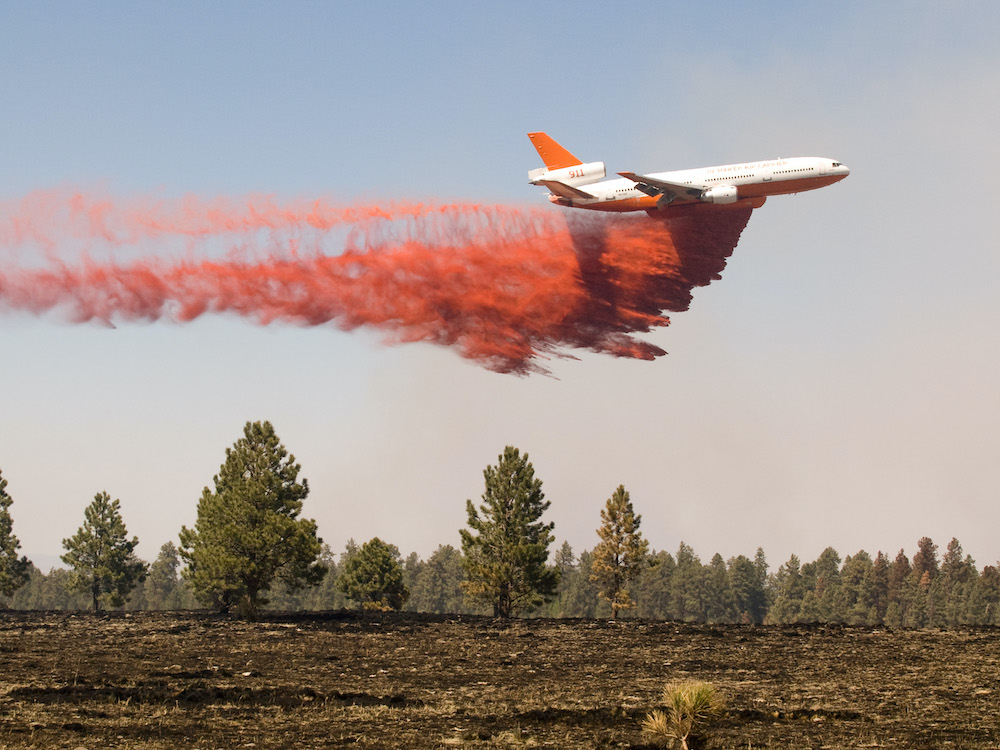
\includegraphics[scale=0.4]{images/dc10.jpg}
  \caption{A DC-10 airtanker, rated for 9,400 gallons, drops retardant above Greer, Arizona.}
\end{figure}

\begin{figure}[h]
  \centering
  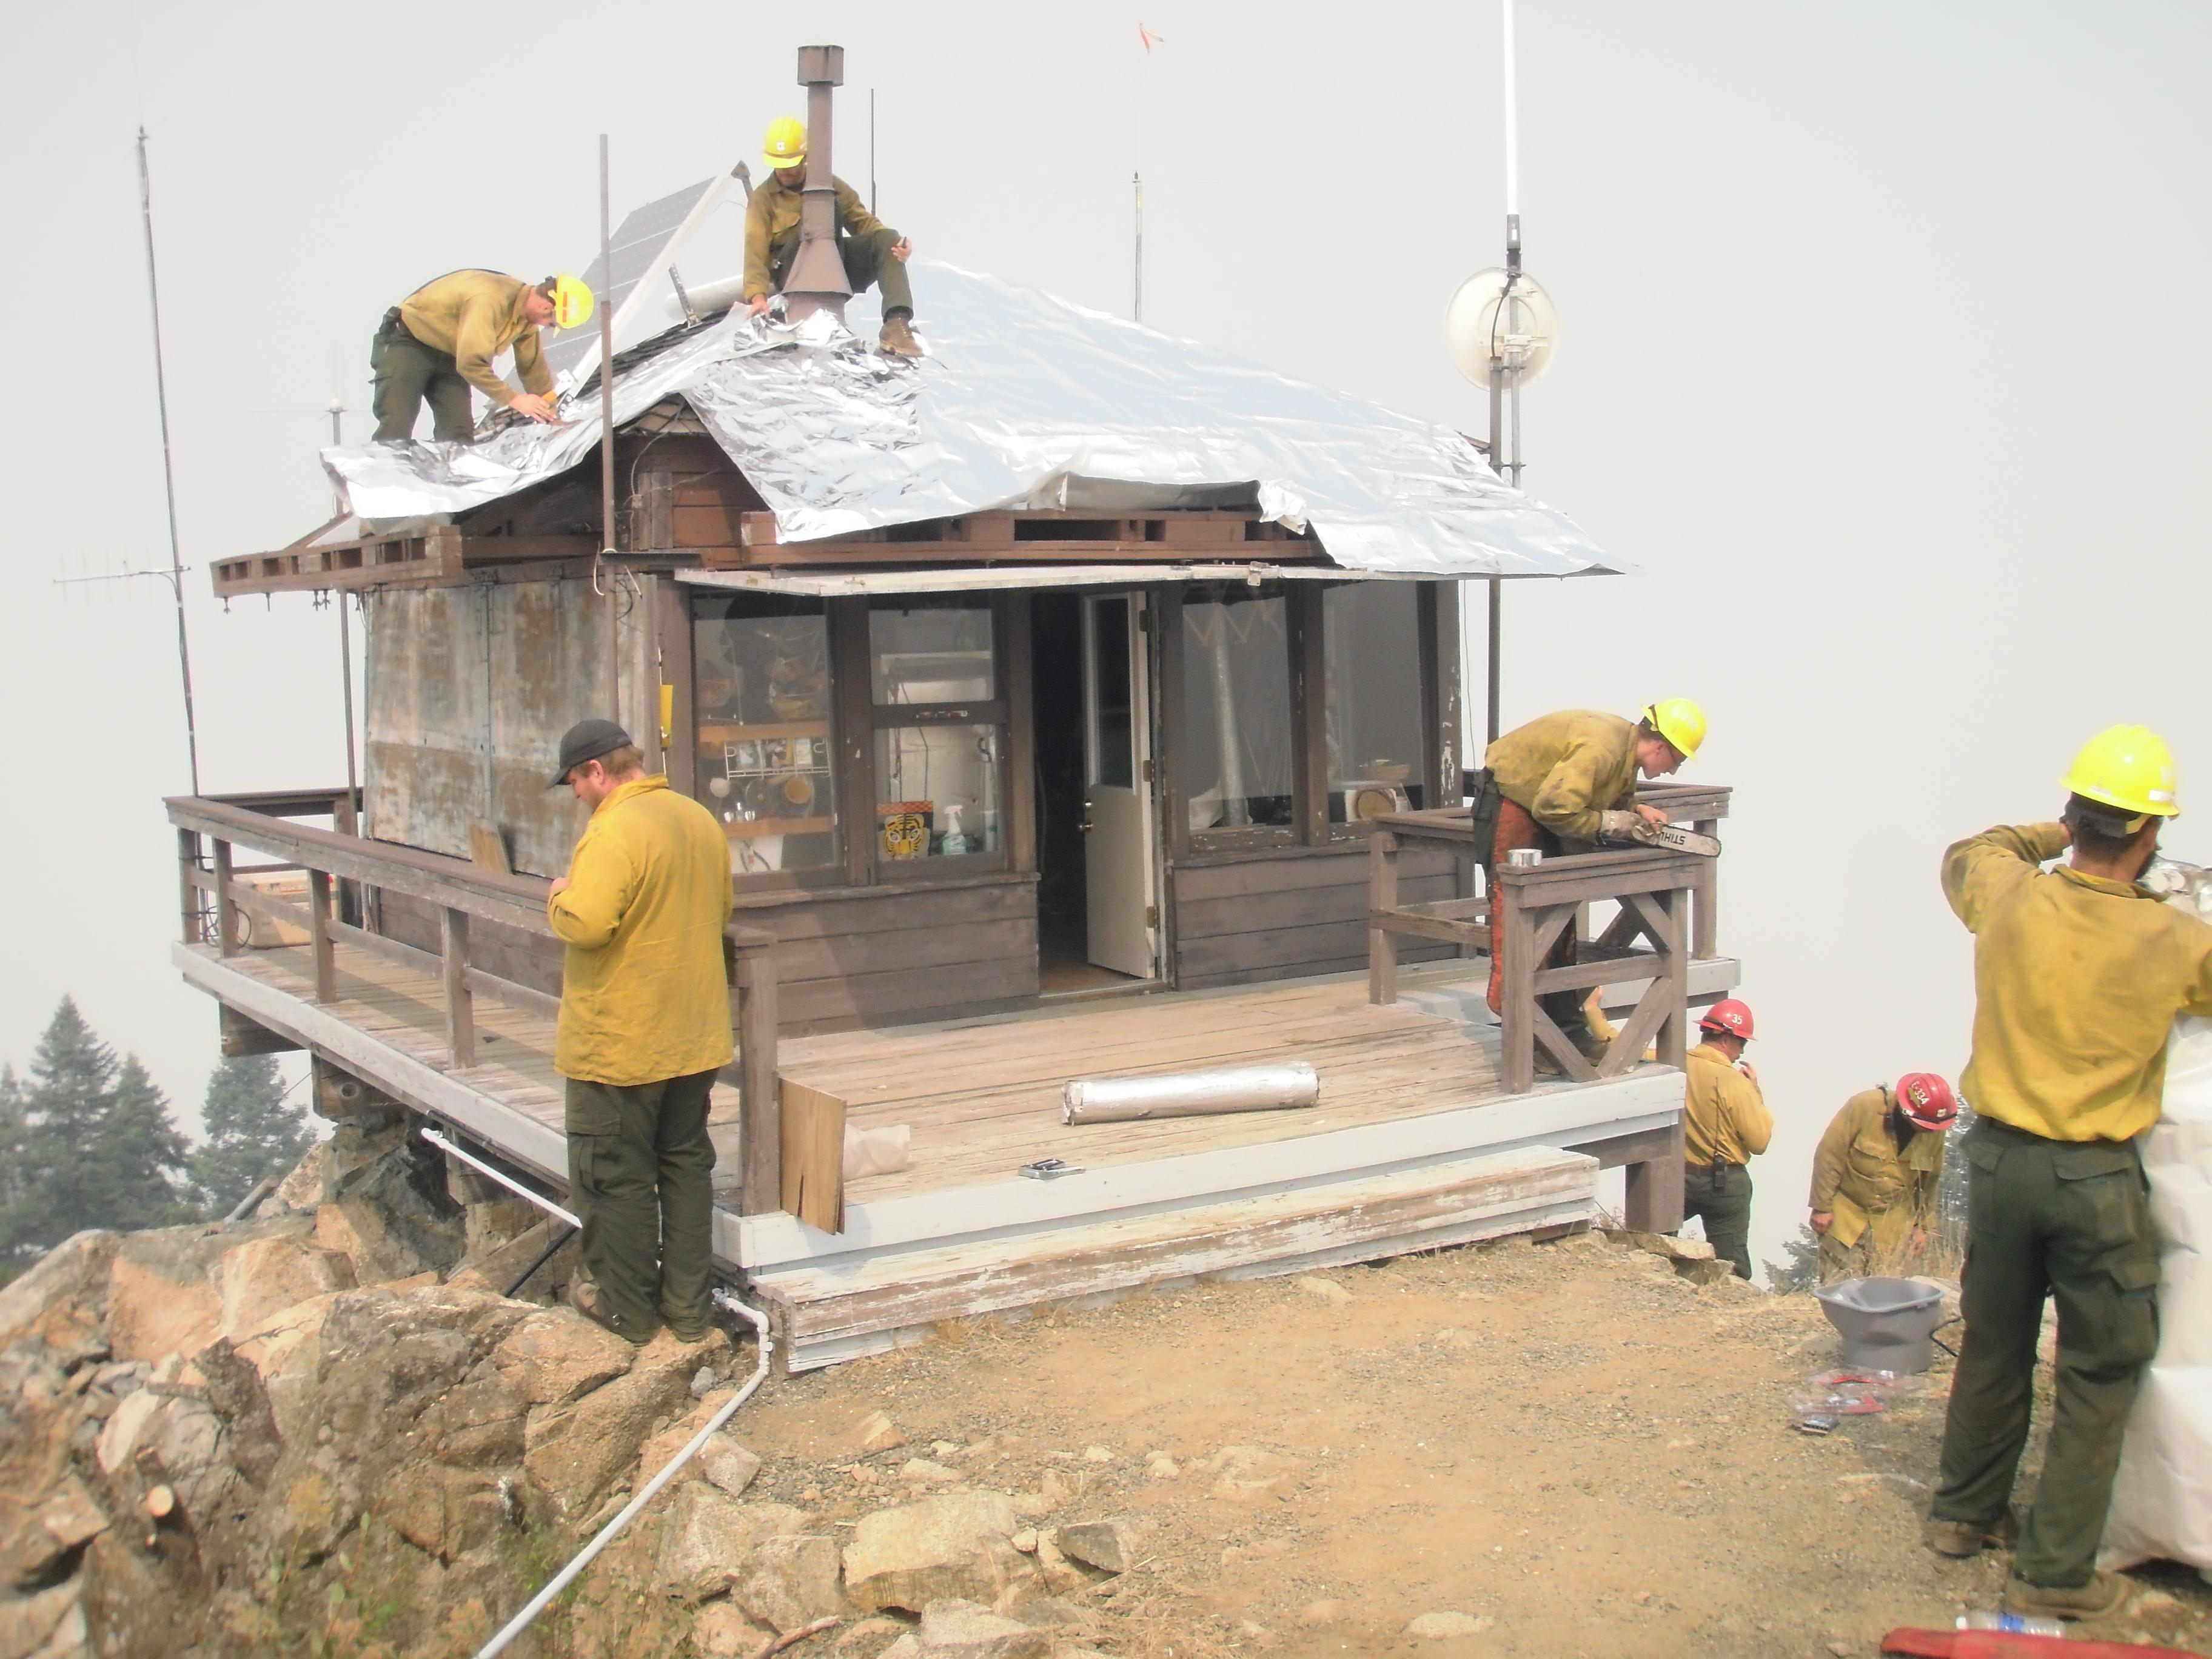
\includegraphics[scale=0.085]{images/ironside.jpg}
  \caption{The Ironside Mountain lookout station, destroyed in the 2021
    Monument fire, shown with protective foil on August
    $10^\textrm{th}$, 2015 during the 2015 River Complex fire. This
    particular fire burned 77,077 acres over 77 days.}
\end{figure}

\subsection{Communication in Practice}\label{communication-in-practice}

Communication patterns in modern wildland firefighting are mostly
simple, even primitive in comparison to what laymen often expect.

In the examples below, we note a kind of ``geospatial locality of
reference'' that system designers should take into account. Generally
speaking, we expect that agents with a higher need to coordinate their
actions will tend to be located closer to each other, which in turn
correlates with an ability to communicate quickly and reliably. This
kind of principle motivates the sort of decentralized, ad-hoc networking
protocols considered in Section \ref{sec:networking}. It can also affect
the design of higher-level applications like the one in Section
\ref{sec:continuous-consistency}

\paragraph{Communication on the ground}

In the field, communication between firefighters and other agents in
disaster response scenarios is often facilitated by handheld (analog)
radios, which are inherently limited in their battery life,\footnote{A
coordinator for NIFS reported that during peak demand, wildland
firefighters in the United States go through upwards of a combined
350,000 ``AA'' batteries in a day.} bandwidth, effective range, and
ability to work around environmental factors like foliage and smoke.

As an alternative to using a radio, it is common for wildland
firefighters in the field to communicate using the simplest of
technologies: shouting back and forth. Besides highlighting the fact
that sometimes simple things work, this is a clear manifestation of
geolocality of reference: firefighters mostly need to communicate when
they are working near each other, in some cases so nearby they can
communicate without network infrastructure.

Communicating over a long distance typically requires infrastructural support, such as the use of cell towers and repeater stations. Typically, disaster
response environments have scarce permanent infrastructure: perhaps a few repeaters mounted to a watch tower for a wildland fire setting. Ad-hoc
infrastructure, such as a cell on wheels (COW) or cell on light truck
(COLT), can sometimes be deployed on an as-needed basis if the location allows for
it. A common issue is making sure that all equipment is properly
configured, for instance that all radios are listening on the correct
frequencies, particularly when different agencies and groups need to
interoperate.

Use of centralized infrastructure comes at the cost of potential
widespread failure when the infrastructure fails. For example, in
California, the Ironside Mountain lookout/repeater station was destroyed
during the 2021 Monument Fire,\footnote{https://www.fire.ca.gov/incidents/2021/7/30/monument-fire/}
which burned approximately 184,142 acres over 88 days. The Ironside
Mountain station had strategic importance, being located on a tall
ridge. According to a video blog from a volunteer firefighter involved
in the incident (CITE), its loss prevented communication between
operators on different sides of the ridge, in networking parlance
creating a \emph{partition} that lasted until crews could ascend the
ridge to deploy a temporary station. This is exactly the kind of
scenario considered by Brewer's CAP theorem in Section
\ref{sec:background}.

\begin{quote}
  When {[}the Ironside Mountain lookout station{]} burned down the radio
  repeater went with it. And so communications were lost across the
  fire\ldots{} one side of the fire couldn't talk to the other side\ldots.
  So it was kind of a critical job to get that road cleared so that the
  radio crews could go back up there and set up a temporary radio tower.
\end{quote}

Large numbers of ground vehicles are involved in wildfire
suppression. A large wildfire response can involve more than 50--100
firetrucks distributed over a large geographical area. Bulldozers and
similar vehicles are commonly used to control the landscape and
perimeter of the fire. An advantage of vehicles is that they can carry
heavier, which is to say better, communications equipment than a
human. For instance, a vehicle could be equipped with a satellite link
as well as a local wireless area network (WLAN) base station, serving
as a bridge between agents in the field and central coordinators
(e.g. incident commanders).

\paragraph{Communication in the air}

Wildland firefighting increasingly involves the use of helicopters and
fixed wing aircraft, but civil aviation has traditionally employed
simpler communication patterns than this use case demands. For instance,
aircraft equipped with Automatic Dependent Surveillance-Broadcast
(ADS-B) monitor their location using GPS and periodically broadcast this
information to air traffic controllers and nearby aircraft. This sort of
scheme has worked well in traditional applications, where pilots
typically only monitor the general locations of a few nearby aircraft.
The locality principle is exhibited here, too: aircraft have the highest
need to coordinate when they are physically close and therefore in range
of each other's ADS-B broadcasts.

In our setting, a large number or aircraft, easily a half dozen or
more, may need to operate in a small area, near complex terrain,
during adverse conditions, often at a low altitude.\footnote{Current
recommendations (WHOSE) call for VLATs to perform drops at 250
ft. above the tree canopy, while smaller aircraft may go lower.} In
other words, the demands are many and the margins for error are
small. This sort of use case requires more sophisticated coordination
schemes between airborne and ground-based elements than solutions like
ADS-B provide by themselves.

As aircraft generally have better line-of-site to ground crews than
ground crews have to each other, firefighters sometimes relay messages
to air-based units over radio, which in turn is relayed back down to
other ground units. The locality principle comes into play here too, but
this time in the reverse direction: this relay scheme allows knowledge
to travel farther, but the extended reach comes at the cost of
introducing delays and possible degradation of message quality, as in
the classic game of telephone.

In some cases, planes from the Civil Air Patrol\footnote{A civil
auxiliary of the U.S. Air Force. https://www.gocivilairpatrol.com/}
(CITE) have been equipped with radio repeaters and dispatched to
wildfires to provide service to ground-based units. In the future, this
sort of service could be provided, perhaps autonomously, by base
stations mounted to unmanned aerial vehicles (UAVs), which might perform
additional functions such as tracking the fire perimeter. More
generally, a future communication system should exploit every pass
messages between agents, even in the event of infrastructure failure, in
a transparent and decentralized fashion. For instance, firefighters may
use an ad-hoc network built from handheld devices, vehicle-mounted
devices, temporary structure, an devices attached to overhead aircraft.
In effect, this would be a high-tech modernization of the sort of
informal relay schemes operating today over traditional radio channels.

\subsection{Towards the Future}\label{towards-the-future}

\begin{itemize}
  \tightlist
\item
  CITE developed a prototype application for firefighters in the field.
\item
  Talk about other applications
\end{itemize}

Taking a broader view, agents in disaster response environments will
often be both producers and consumers of data, and this data will need
to processed for agents to make informed decisions. Our background
research indicated many different kinds of data that could be valuable
for responders. To give just a glimpse:

\begin{itemize}
  \tightlist
\item
  Free-form communication, especially recorded voice messages to be
  broadcast to many firefighters at once.
\item
  The exact or estimated location of firefighters, vehicles, victims,
  hazards, etc.
\item
  Medical information, perhaps collected from digital triage tags (CITE)
\item
  Data about current and predicted fire or weather patterns
\item
  Topographic information about the terrain, highlighting for instance
  the location of rivers and roads that could form a fire control line
\item
  Planned escape routes, safety zones, and landing zones
\item
  Availability and dispatching of resources, e.g.~ambulances,
  airtankers, or crews on standby
\end{itemize}

In a perfect environment, such information would be shared with all
necessary agents in whole and instantly. In reality, agents will be
presented with information that is sometimes incomplete, out of date, or
contradictory---all problems that are further exacerbated by an
unreliable network.

For instance, a central data fusion center may be used to detect and
alert responders to a fire that has accidentally moved beyond a control
line (known as \emph{slopover}). Such information would be of high
importance, and it would be worthwhile to expend network resources
conveying this information to the relevant parties. On the other hand, a
firefighter may not need the minute GPS position of every other
firefighter in the field: perhaps the exact location of teammates, and
the general location of other crews.

Warn firefighters when they are too far from an escape route or safety zone.

For developers, it is clear that this requires some coordination between
the application and the networking layers, as the latter must be given
enough information to make the most prudent use of limited resources.

\newpage

\section{Introduction to Distributed
  Systems}\label{introduction-to-distributed-systems}

\label{sec:background}

A distributed system, in the most general sense, is a collection of
independent entities that cooperate to solve a problem that cannot be
individually solved \cite{kshemkalyani_singhal_2008}. Singhal and
Shivaratri \cite{10.5555/562065} offer the following definition of a
distributed (computing) system:

\begin{quote}
  ``A collection of computers that do not share common memory or a common
  physical clock, that communicate by message passing over a communication
  network, and where each computer has its own memory and runs its own
  operating system.''
\end{quote}

In our scenarios, system nodes typically represent computers, routers,
sensors, and communication devices, while the clients would typically be
firefighters using these devices and other persons involved in disaster
response efforts. The components of the system coordinate to solve such
tasks as navigating safely in close proximity, delivering resources to
remote locations, suppressing fires, or measuring environmental
conditions.

A fundamental goal for distributed computing systems is to
``{[}appear{]} to the users of the system as a single coherent
computer'' \cite{TanenbaumSteen07}. This can be understood as the
requirement that all nodes present a \emph{mutually-consistent} view of
the world, e.g.~the state of a globally-maintained database, to system
clients. Bad things happen when consistency is violated:

\begin{itemize}
\item
  If two air traffic controllers were presented with conflicting
  information about the trajectory of aircraft, they could potentially
  issue dangerously incongruous instructions to pilots.
\item
  Messages between users that are delivered in the wrong order can lead
  to misunderstandings.
\item
  A bank client would be unhappy if deposits that appear in their
  account online are not reflected when they check their balance at an
  ATM, or if they seem to disappear after refreshing the webpage.
\item
  Resource-tracking systems are not useful if a resource that appears to
  be available cannot be used because the information is out of date, or
  a resource that is actually available cannot be used because clients
  think it is still unavailable.
\end{itemize}

Enforcing consistency means clients are presented with the abstraction
of a shared world, as if they are all connected to a central computer
rather than a complex system of loosely coupled independent computers.
This abstraction shields users and developers from complexity and makes
it simpler to reason about a system's behavior. Violating consistency
means the abstraction of a shared universe is broken, which can
invalidate clients' mental model of the system, make the system's
behavior harder to predict, or cause safety requirements to be violated.

Clearly, all other things being equal, one wants distributed systems to
have as much consistency as possible. However, we shall see that strong
notions of consistency are brittle in the sense that they generally
cannot be achieved for the kinds of systems we consider in this
document. In practical applications this implies that tradeoffs will
have to be made \emph{somewhere}, so it is necessary to understand where
this happens and make choices informed both by general systems theory
and the particulars of the real environment and use case.

\subsection{Message Passing}\label{message-passing}

A distributed system consists of a set
\(\mathcal{P} = \{P_i\}_{i\in I}\) of \emph{processes}, which we think
of these as executing on independent, often geographically dispersed
computers that communicate by message-passing. Processes can \emph{only}
coordinate by passing messages over the network. This fact is implied by
absence of a common memory, whereas processes on the same machine have
the option to share data by writing it to a memory location both
processes have access to.

A foundational assumption is that the network is almost always less than
perfectly reliable---this fact can be counted on during emergencies.
Imperfection means that message delivery is not instantaneous may be
unpredictable. The network may deliver a packet zero times (i.e.~it may
silently delete the packet) or multiple times, and furthermore different
packets may arrive in any order.\footnote{In the case of \emph{Byzantine
faults} (CITE) the network may even act like a malicious adversary,
though we will not consider this scenario in this document.} All of
these behaviors represent obstructions to consistency and make it
challenging to enforce safety requirements. We shall now make this
discussion more precise.

\hypertarget{client-server-architecture}{%
  \subsubsection{Client-server
    architecture}\label{client-server-architecture}}

Process take requests from clients, such as to read or write a value in
a database. The lifecycle of a typical request is depicted in Figure
\ref{fig:request}. At some physical time (i.e.~wall-clock time)
\(C.s \in \mathbb{R}\) (client start time), a client sends a message to
a process. At time \(E.s\), which we'll call the \emph{start time} of
the event, the message is accepted by the process. The request is
processed until some strictly greater time \(E.t > E.s\) when a response
is sent back to the client. The value \(E.t - E.s\) is the
\emph{duration} of the event.

\begin{figure}[h]
  \center
  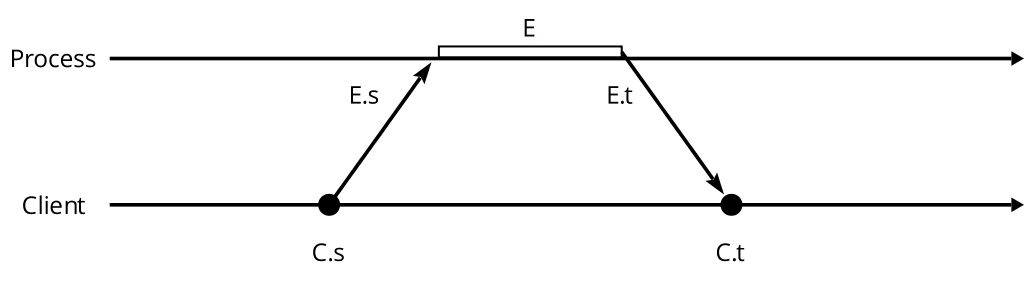
\includegraphics[scale=0.4]{images/request.png}
  \caption{Lifetime of a client request}
  \label{fig:request}
\end{figure}

While handling the request, the process may coordinate with other
processes in the background by sending and receiving more messages. For
example, the process may propagate the client's request to other
processes, retrieve up-to-date values from other processes to give to
the client, or delay handling the client's request in order to handle
other requests.

\subsubsection{Causal precedence/``happens before''/external
  order}\label{causal-precedencehappens-beforeexternal-order}

As is often the case, we shall assume that requests handled by a single
process do not overlap in time. This can be enforced with local
serialization methods such as two-phase locking (CITE) that can be used
to isolate concurrent transactions from each other, providing the
abstraction of a system that handles requests one at a time. On the
other hand, any two processes may handle two events at the same physical
time, so that there is no obvious total order of events across the
system. Instead, one has a partial order called \emph{external order}.
Intuitively, it is the partial order of events that would be witnessed
by an observer recording the real time at which systems begin and finish
responding to requests.

\begin{definition}
  Let $E$ be an execution. Request $E1$ \emph{externally precedes}
  request $E2$ if $E1.t < E2.s$. That is, if the first request
  terminates before the second request is accepted. This induces an
  irreflexive partial order called \emph{external order}.
\end{definition}

Recall that an irreflexive partial order is a binary relation \(<\) such
that \(A \not < A\), \(A < B \implies B \not < A\), and
\(A < B, B < C \implies A < C\).

Because we assume processes handle events one-at-a-time, the events
handled at any one process are totally ordered by external order---one
event cannot start before another has finished. If \(E1\) and \(E2\) are
events at \emph{different} processes, they need not be comparable by
external order, i.e.~neither \(E1.t < E2.s\) nor \(E2.t < E1.s\), making
them \emph{physically concurrent}.

\begin{definition}
  If two events overlap in physical time
  (equivalently, if they are not comparable by external order), we call the events \emph{physically concurrent} and
  write $E1 || E2$.
\end{definition}

Physical concurrency is a reflexive and symmetric---but usually not
transitive--- binary relation. Such structures are often called
\emph{compatibility relations.} The general intuition is that anything
is compatabile with itself (reflexivity), and the compatibility of two
objects does not depend on their order (symmetry). But if \(A\) and
\(B\) are compatible with \(C\), it need not be the case that \(A\) and
\(B\) are compatible with each other.

Figure \ref{fig:externalorderexec} shows the external order relation for
an execution. To save space we elide arrows between two events of the
same process and arrows that can be inferred by transitivity. This
corresponds to the directed acyclic graph structure shown in
\ref{fig:externalorderdag}.

\begin{figure}
  \begin{subfigure}[a]{1\textwidth}
    \center
    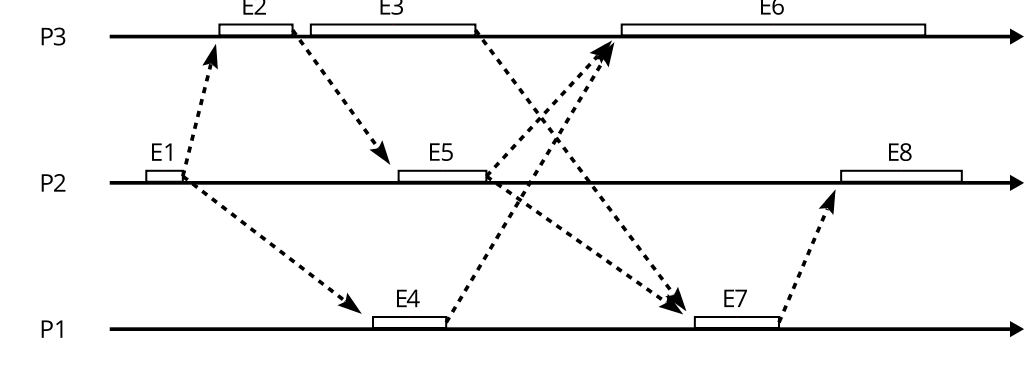
\includegraphics[scale=0.4]{images/externalorder.png}
    \caption{Depiction of external order between concurrent events across three processes. Intra-process and transitive edges are not depicted.}
    \label{fig:externalorderexec}
  \end{subfigure}
  \begin{subfigure}[b]{1\textwidth}
    \center
    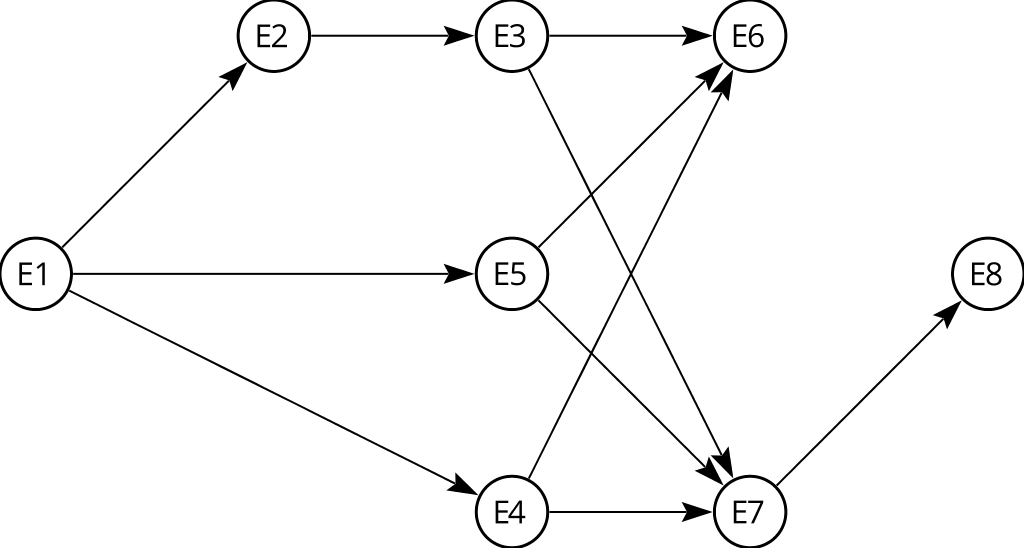
\includegraphics[scale=0.25]{images/partialorder.png}
    \caption{The directed acyclic graph (DAG) induced by external order.}
    \label{fig:externalorderdag}
  \end{subfigure}
  \caption{External order}
  \label{fig:externalorder}
\end{figure}

The reader may wonder if we can consider events to be totally ordered,
say by pairing them with a timestamp that records their physical start
time to resolve ties like \(x || y\). This order is not generally useful
for a couple reasons. First, we assume processes have only loosely
synchronized clocks, so timestamps from two different processes may not
be comparable. Additionally, even systems that enforce linearizable
consistency (c.f. Section \ref{sec:atomic}) do not necessarily handle
requests in order of their physical start times.

\subsection{Memory Consistency Models}\label{memory-consistency-models}

\label{sec:atomic}

What precisely constitutes consistency? One can choose from multiple
consistency models, and the most appropriate model depends on the
semantics expected by the application and its clients, which must be
weighed against other requirements.

To discuss consistency models, we shall be less interested in the
details of message-passing and more interested just in the responses
observed by clients. We shall consider the full set of events across a
distributed system, such as shown in Figure \ref{fig:externalorder}.
This is called an \emph{execution}. Consistency models constrain the set
of allowable return values in response to clients' requests.

A fundamental distributed application is the \emph{shared distributed
memory} abstraction. We shall assume that all processes maintain a local
replica of a globally shared data object, as replication increases
system fault tolerance. For simplicitly, we shall discuss the data store
as a simple key-value store, but it could be something else like a
database, filesystem, persistent object, etc.

We assume clients submit two types of requests to processes. A
\emph{read request} is a request to lookup the current value of a
variable. A request to read the variable \(x\) that returns value \(a\)
is written \(R(x,a)\). A \emph{write request} is a request to set the
current value of a variable. Notation \(W(x,a)\) represents writing
value \(a\) to \(x\). We assume all processes provide access to the same
set of shared variables.

A \emph{memory consistency model} formally constrains the allowable
system responses during executions. \emph{Strong} consistency models are
generally understood as ones provide the illusion that all clients are
accessing just one globally shared replica. As we will see, this still
leaves room for different possible behaviors (i.e.~allows
non-determinism in the execution of a distributed application), but the
allowable behavior is tightly constrained.

\hypertarget{linearizabilityatomic-consistency}{%
  \subsubsection{Linearizability/atomic
    consistency}\label{linearizabilityatomic-consistency}}

\emph{Linearizability} (Herlihy and Wing 1990) is essentially the
strongest common consistency model. It is known variously as atomic
consistency, strict consistency, and sometimes external consistency. In
the context of database transactions (which come with other guarantees,
like isolation, that are more specific to databases), the analogous
condition is called strict serializability. A linearizable execution is
defined by three features:

\begin{itemize}
  \tightlist
\item
  All processes act like they agree on a single, global total order
  defined across all accesses.
\item
  This sequential order is consistent with the actual external order.
\item
  Responses are semantically correct, meaning a read request \(R(x, a)\)
  returns the value of the most recent write request \(W(x, a)\) to
  \(x\).
\end{itemize}

\begin{figure} \begin{subfigure}[a]{1\textwidth} \center
    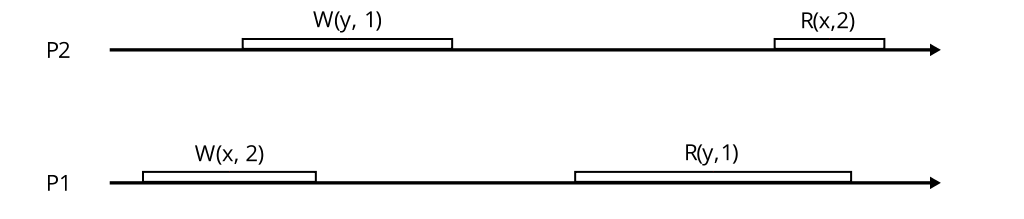
\includegraphics[scale=0.4]{images/linear1.png} \caption{A
      linearizable execution. Any choice of linearization works here.}
    \label{fig:linear_example11} \end{subfigure}
  \begin{subfigure}[b]{1\textwidth} \center
    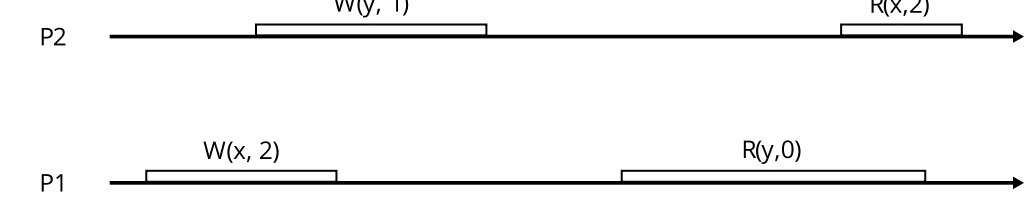
\includegraphics[scale=0.4]{images/nonlinear0.png} \caption{A
      non-linearizable execution. The request to read $y$ returns a
      stale value. } \label{fig:linear_example12} \end{subfigure}
  \caption{A linearizable and non-linearizable execution.}
  \label{fig:linear_example1} \end{figure}

Figure \ref{fig:linear_example11} shows a prototypical example of a
linearizable execution. We assume that all memory locations are
initialized to \(0\) at the system start time. Intuitively, it should
appear to an external observer that each access instantaneously took
effect at some point between its start and end time. Hence, the request
to read the value of \(y\) returns \(1\), because at some point between
\(W(y,1).s\) and \(W(y,1).t\) that change took effect. If client on
\(P_1\) read a stale value, we would say the execution is not
linearizable. Figure \ref{fig:linear_example12} shows an
non-linearizable execution that returns stale data instead of reflecting
the write access to \(y\) on \(P2\).

Linearizability can be precisely defined in terms of
\emph{linearizations.}

\begin{definition}
  A \emph{linearization point} $t \in \mathbb{R} \in [E.s, E.t]$ for an
  event $E$ is a time between the event's start and termination. An
  execution is \emph{linearizable} if and only if there is a choice of
  linearization point for each access, which induces a total order called a \emph{linearization},
  such that $E$ is equivalent to
  the serial execution of events when totally ordered by their
  linearization points.
\end{definition}

\begin{figure}[p]
  \begin{subfigure}[a]{1\textwidth}
    \center
    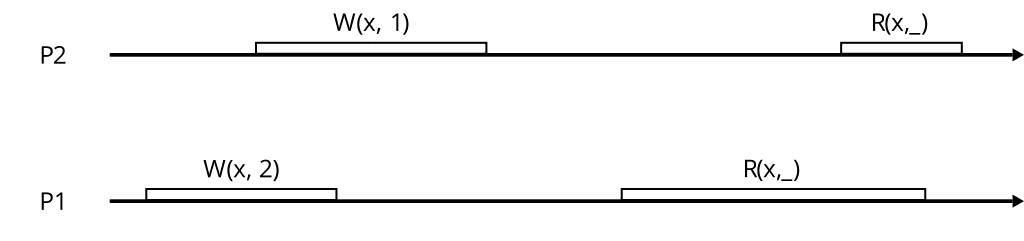
\includegraphics[scale=0.4]{images/linearTemplate.png}
    \caption{An execution with read responses left unspecified.}
    \label{fig:nonlinear}
  \end{subfigure}
  \begin{subfigure}[b]{1\textwidth}
    \center
    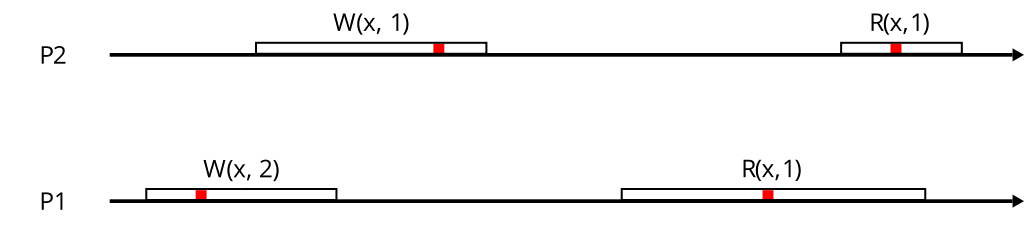
\includegraphics[scale=0.4]{images/linear3.png}
    \caption{A linearizable execution for which both reads return $1$.}
  \end{subfigure}
  \begin{subfigure}[c]{1\textwidth}
    \center
    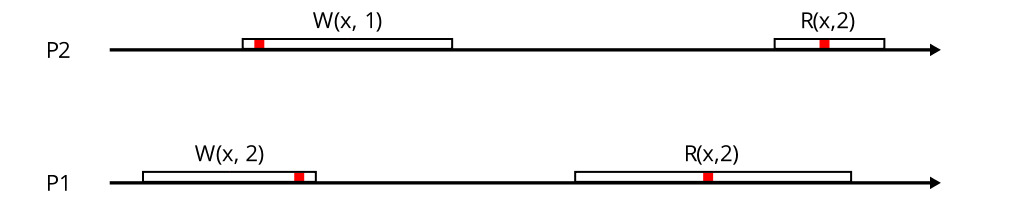
\includegraphics[scale=0.4]{images/linear2.png}
    \caption{A linearizable execution for which both reads return $2$.}
  \end{subfigure}
  \caption{Two linearizable executions of the same underlying events that return different responses. Possible linearization points are shown in red.}
  \label{fig:linearization}
\end{figure}

\begin{figure}[p]
  \begin{subfigure}[a]{1\textwidth}
    \center
    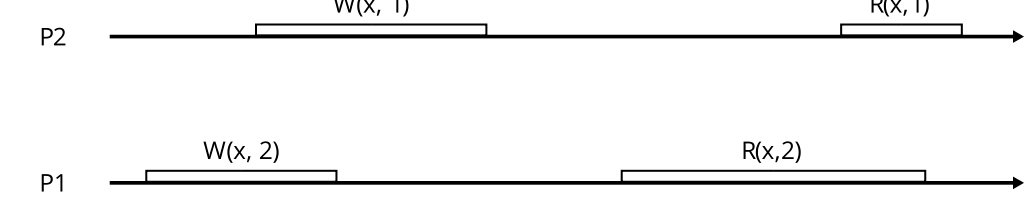
\includegraphics[scale=0.4]{images/nonlinear1.png}
    \caption{A nonlinearizable execution with the read access returning disagreeing values. We will see later (Figure \ref{fig:sequential}) that this execution is still sequentially consistent. }
    \label{fig:nonlinear1}
  \end{subfigure}
  \begin{subfigure}[b]{1\textwidth}
    \center
    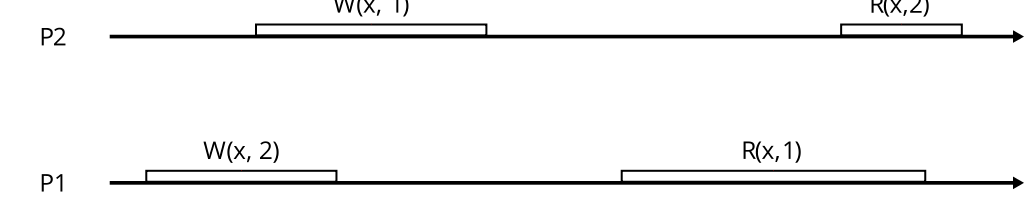
\includegraphics[scale=0.4]{images/nonlinear2.png}
    \caption{Another nonlinearizable execution with read access values swapped. This execution is not sequentially consistent.}
    \label{fig:nonlinear2}
  \end{subfigure}
  \caption{Two non-linearizable executions of the same events shown in Figure \ref{fig:linearization}.}
  \label{fig:nonlinearizable}
\end{figure}

Linearization points are demonstrated in Figure \ref{fig:linearization}.
The figure shows different linearizable behaviors in response to the
same underlying set of accesses. It is assumed no distinct access can
have the same linearization point, so that we get a total order. This
demonstrates that linearizability still leaves some room for
non-determinism in the execution of distributed applications. In this
example, the requests must both return 1 or 2. The constraint is that
the values must agree---linearizability forbids the situation in which
one client reads \(1\) and another reads \(2\) (Figure
\ref{fig:nonlinearizable}).

\begin{definition}
  We say an entire system is linearizable when all
  possible executions of the system are linearizable.
\end{definition}

\hypertarget{sequential-consistency}{%
  \subsubsection{Sequential consistency}\label{sequential-consistency}}

Enforcing atomic consistency means that an access \(E\) at process
\(P_i\) cannot return to the client until every other process has been
informed about \(E\). For many applications this is an unacceptably high
penalty. A weaker model that is still strong enough for most purposes is
\emph{sequential} consistency. This is an appropriate model if a form of
strong consistency is required, but the system is agnostic about the
precise physical time at which events start and finish, provided they
occur in a globally agreed upon order.

A sequentially consistent system ensures that any execution is
equivalent to some global serial execution, even if this is serial order
is not the one suggested by the real-time ordering of events. When
real-time constraints are not important, this provides essentially the
same benefits as linearizability. For example, it allows programmers to
reason about concurrent executions of programs because the result is
always guaranteed to represent some possible interleaving of
instructions, never allowing instructions from one program to execute
out of order.

\begin{definition}
  \label{def:sequentiallyconsistent}
  A \emph{sequentially consistent} execution is
  characterized by three features:
  \begin{itemize}
  \item All processes act like they agree on a single, global total order
    defined across all accesses.
  \item This sequential order is consistent with the program order of each process.
  \item Responses are semantically correct, meaning reads return the most recent writes (as determined by the global order)
  \end{itemize}
\end{definition}

Processes in a sequentially consistent system are required to agree on a
total order of events, presenting the illusion of a shared database from
an application programmer's point of view. However, this order need not
be given by external order. Instead, the only requirement is that
sequential history must agree with process order, i.e.~the events from
each process must occur in the same order as in they do in the process.
This is nearly the definition of linearizability, except that external
order has been replaced with merely program order. We immediately get
the following lemma.

\begin{lemma}
  \label{lem:linearsequential}
  A linearizable execution is sequentially consistent.
\end{lemma}
\begin{proof}
  This follows because process order is a subset of external order.
\end{proof}

\begin{figure}
  \begin{subfigure}[a]{1\textwidth}
    \center
    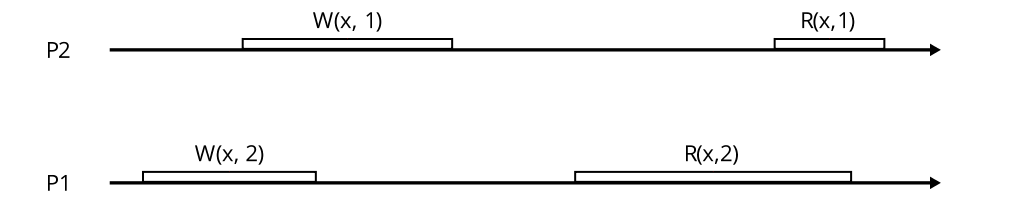
\includegraphics[scale=0.4]{images/sequential1.png}
    \caption{A non-linearizable, sequentially consistent execution.}
    \label{fig:sequential1}
  \end{subfigure}
  \begin{subfigure}[b]{1\textwidth}
    \center
    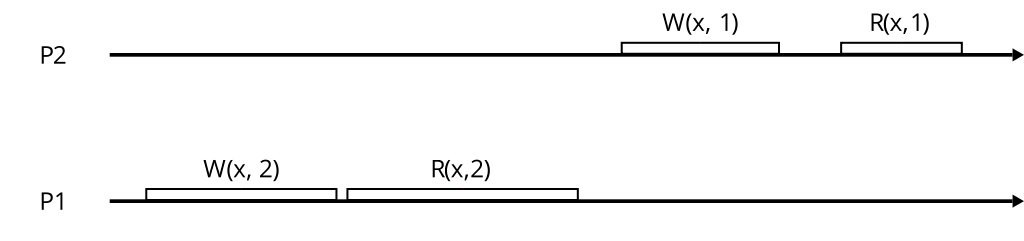
\includegraphics[scale=0.4]{images/sequential2.png}
    \caption{An equivalent interleaving of \ref{fig:sequential1}.}
    \label{fig:interleaving1}
  \end{subfigure}
  \caption{A sequentially consistent execution and a possible interleaving.}
  \label{fig:sequential}
\end{figure}

Visually, sequential consistency allows reordering an execution by
sliding events along each process' time axis like beads along a string.
Two events from the same process cannot pass over each other as this
would violate program order, but events on different processes may be
commuted past each other, violating external order. This sliding allows
defining an arbitrary interleaving of events, a totally ordered
execution with no events overlapping. From this perspective, while
linearizability requires the existence of a linearization, sequential
consistency requires the existence of an equivalent interleaving.

The converse of Lemma \ref{lem:linearsequential} does not hold. For
example, Figure \ref{fig:sequential1} was previously shown (Figure
\ref{fig:nonlinear1}) as a nonlinearizable execution. However, it is
sequentially consistent, as evidenced by the interleaving in Figure
\ref{fig:interleaving1} that slides the events \(W(x,1)\) and \(R(x,2)\)
past each other.

\begin{figure}
  \begin{subfigure}[a]{1\textwidth}
    \center
    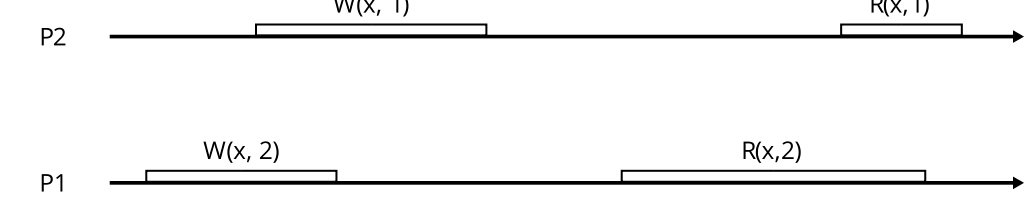
\includegraphics[scale=0.4]{images/nonsequential1.png}
    \caption{A non-sequentially consistent execution.}
    \label{fig:nonsequential1}
  \end{subfigure}
  \begin{subfigure}[b]{1\textwidth}
    \center
    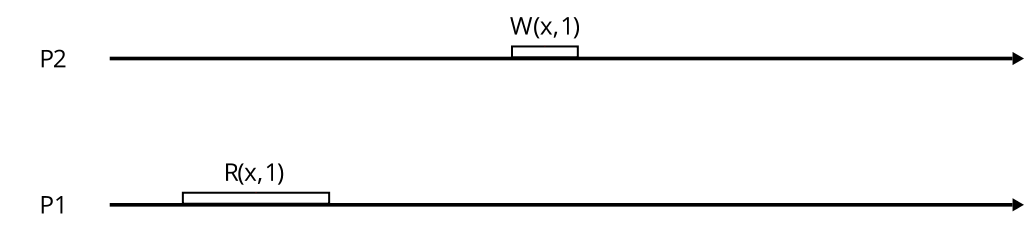
\includegraphics[scale=0.4]{images/nonsequential_x.png}
    \caption{The sequentially consistent history of $x$.}
    \label{fig:sequentialx}
  \end{subfigure}
  \begin{subfigure}[b]{1\textwidth}
    \center
    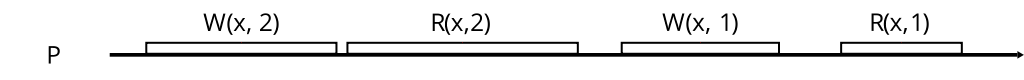
\includegraphics[scale=0.4]{images/nonsequential_y.png}
    \caption{The sequentially consistent history of $y$.}
    \label{fig:sequentialy}
  \end{subfigure}
  \caption{A non-sequentially consistent execution with sequentially-consistent executions at each variable.}
  \label{fig:nonsequential}
\end{figure}

\hypertarget{causal-consistency}{%
  \subsubsection{Causal consistency}\label{causal-consistency}}

Suppose in a message stream two questions \(Q_1\) and \(Q_2\) are asked
and responses \(A_1\) and \(A_2\) are given, respectively. If the
answers arrive in the wrong order, i.e.~\(A_2\) appears as the answer to
\(Q_1\) and vice versa, the potential for confusion can be severe.

\hypertarget{the-cap-theorem}{%
  \subsection{The CAP Theorem}\label{the-cap-theorem}}

Real-world systems often fall short of behaving as a single perfectly
coherent system. The root of this phenomenon is a deep and
well-understood tradeoff between system coherence and performance.
Enforcing consistency comes at the cost of additional communications,
and communications impose overheads, often unpredictable ones.

Fox and Brewer \cite{1999foxbrewer} are crediting with observing a
particular tension between the three competing goals of consistency,
availability, and partition-tolerance. This tradeoff was precisely
stated and proved in 2002 by Gilbert and Lynch
\cite{2002gilbertlynchCAP}.  The theorem is often somewhat
misunderstood, as we discuss, so it is worth clarifying the terms
used.

\paragraph{Consistency}

Gilbert and Lynch define a consistency system as one whose executions
are always linearizable.

\paragraph{Availability}

A CAP-available system is one that will definitely respond to every
client request at some point.

\paragraph{Partition tolerance}

A partition-tolerant system continues to function, and ensure whatever
guarantees it is meant to provide, in the face of arbitrary partitions
in the network (i.e., an inability for some nodes to communicate with
others). It is possible that a partition never recovers, say if a
critical communications cable is permanently severed.

A partition-tolerant CAP-available system cannot indefinitely suspend
handling a request to wait for network activity like receiving a
message. In the event of a partition that never recovers, this would
mean the process could wait indefinitely for the partition to heal,
violating availability. On the other hand, a CAP-consistent system is
not allowed to return anything but the most up-to-date value in response
to client requests. Keep in mind that any (other) process may be the
originating replica for an update. Some reflection shows that the full
set of requirements is unattainable---a partition tolerant system simply
cannot enforce both consistency and availability.

\begin{theorem}[The CAP Theorem]
  \label{thm:cap}
  In the presense of indefinite network partitions, a distributed system
  cannot guarantee both linearizability and eventual-availability.
\end{theorem}
\begin{proof}
  Technically, the proof is almost trivial. We give only the informal
  sketch here, leaving the interested reader to consult the more formal
  analysis by Gilbert and Lynch. The key technical assumption is that a
  processes' behavior can only be influenced by the messages it actually
  receives---it cannot be affected by messages that are sent to it but
  never delivered.

  In Figure \ref{fig:linear_example11}, suppose the two processes are on
  opposite sides of a network partition, so that no information can be
  exchanged between them (even indirectly through a third party). If we
  just consider the execution of $P_2$ by itself, without $P_1$,
  linearizability would require it to read the value $2$ for $y$. If we
  do consider $P_1$, linearizability requires that the read access to
  $y$ must return $1$. But if $P_2$ cannot send messages to $P_1$, then
  $P_2$'s behavior cannot be influenced by the write access to $y$, so
  it would still have to return $2$, violating
  consistency. Alternatively, it could delay returning any result until
  it is able to exchange messages with $P_1$. But if the partition never
  recovers, $P_1$ will wait forever, violating availability.
\end{proof}

\paragraph{CAP for Sequential Consistency}

Sequential consistency is a relaxation of atomic consistency, but not by
much. The model is still too strict to enforce under partition
conditions.

\begin{lemma}[CAP for sequential consistency]
  \label{thm:cap-sequential}
  An eventually-available system cannot provide sequential consistency in the presense of network partitions.
\end{lemma}
\begin{proof}

  The proof is an adaptation of Theorem \ref{thm:cap}. Suppose $P_1$ and
  $P_2$ form of CAP-available distributed system and consider the
  following execution: $P_1$ reads $x$, then assigns $y$ the value
  $1$. $P_2$ reads $y$, then assigns $x$ the value $1$. (Note that this
  is the sequence of requests shown in Figure \ref{fig:nonsequential1},
  but we make no assumptions about the values returned by the read
  requests). By availability, we know the requests will be handled (with
  responses sent back to clients) after a finite amount of time. Now
  suppose $P_1$ and $P_2$ are separated by a partition so they cannot
  read each other's writes during this process. For contradiction,
  suppose the execution is equivalent to a sequential order.

  If $W(y,1)$ precedes $R(y)$ in the sequential order, then $R(y)$ would
  be constrained to return to $1$. But $P_2$ cannot pass information to
  $P_1$, so this is ruled out. To avoid this situation, suppose the
  sequential order places $R(y)$ before $W(y,1)$, in which case $R(y)$
  could correctly return the initial value of $0$. However, by
  transitivity the $R(x)$ event would occur after $W(x,1)$ event, so it
  would have to return $1$. But there is no way to pass this information
  from $P_1$ to $P_2$. Thus, any attempt to consistently order the
  requests would require commuting $W(y,1)$ with $R(x)$ or $W(x,1)$ with
  $R(y)$, which would violate program order.
\end{proof}


\hypertarget{interpretation-of-the-cap-theorem}{%
  \subsubsection{Interpretation of the CAP
    Theorem}\label{interpretation-of-the-cap-theorem}}

While the proof of the CAP theorem is simple, its interpretation is
subtle and has been the subject of much discussion in the years since
\cite{2012CAP12Years}. It is sometimes assumed that the CAP theorem claims that
a distributed system can only offer two of the properties C, A, and P.
In fact, the theorem constrains, but does not prohibit the existence of,
applications that apply some relaxed amount of all three features. The
CAP theorem only rules out their combination when all three are
interpreted in a highly idealized sense.

In practice, applications can tolerate much weaker levels of consistency
than linearizability. Furthermore, network partitions are usually not as
dramatic as an indefinite communications blackout. Real conditions in
our context are likely to be chaotic, featuring many smaller disruptions
and delays and sometimes larger ones. Communications between different
clients may be affected differently, with nearby agents generally likely
to have better communication channels between them than agents that are
far apart. Finally, CAP-availability is a suprisingly weak condition.
Generally one cares about the actual time it takes to handle user
requests, but the CAP theorem exposes difficulties just ensuring the
system handles requests at all. Altogether, the extremes of C, A, and P
in the CAP theorem are not the appropriate conditions to apply to many,
perhaps most, real-world applications.

\paragraph{The safety/liveness tradeoff}

The tension between consistency and availability is a prototypical
example of a deeper tension in computing: that between safey and
liveness properties \cite{10.1145/5505.5508 2012perspectivesCAP}. These terms can be understood as follows.

\begin{itemize}
\item
  \textbf{Safety} properties ensure that a system avoids doing something
  ``bad'\,' like violating a consistency invariant. Taken to the
  extreme, one way to ensure safety is to do nothing. For instance, we
  could enforce safety by never responding to read requests in order to
  avoid offering information that is inconsistent with that of other
  nodes.
\item
  \textbf{Liveness} properties ensure that a system will eventually do
  something ``good'\,', like respond to a client. Taken to the extreme,
  one very lively behavior would be to immediately respond to user
  requests, without taking any steps to make sure this response is
  consistent with that of other nodes.
\end{itemize}

Note that ``safety'' is narrow sense, meaning a constraint on a system's
allowable responses to clients, while liveness properties require the
system to ``do'' something instead of delaying forever. Clearly, it is
important for systems in safety-related applications to have some amount
of liveness, and not just ``safety'' properties. Liveness and safety are
both good.

Because of the tension between them, building applications that provide
both safety and liveness features is challenging. The fundamental
principle is that if we want to increase how quickly a system can
respond to requests, eventually we must relax our constraints on what
the system is allowed to return.

\newpage

\hypertarget{desiderata}{%
  \section{Desiderata}\label{desiderata}}

\subsection{Assumptions}

\begin{itemize}
\item Only very loose clock synchronization. However, we may fairly assume that nodes can measure the passage of time. Real timestamps may be collected on data (for example, for later analysis), but the correct configuration of these clocks cannot be relied upon, particularly at lower levels of abstraction.
\item
\end{itemize}

\subsection{Desiderata}

\label{sec:desiderata}

Having discussed some of the fundamental distributed systems issues that
arise under real-world network conditions, we turn our attention to
three desiderata we will use to frame and analyze the models discussed
in Sections \ref{sec:continuous-consistency} and \ref{sec:data-fusion}.

The CAP theorem, and others like it, place fundamental limitations on
the consistency of real-world distributed systems. In the absense of a
``perfect'' system, engineers are forced to make tradeoffs. Ideally,
these tradeoffs should be tuned for the specific application in mind---a
protocol that works well in a datacenter might not work well in a
heterogeneous geodistributed setting. This section lists three desirable
features of distributed systems and frameworks for reasoning about or
implementing them. We chose this set based on the particular details of
civil aviation and disaster response, where safety is a high priority
and usage/communication patterns may be unpredictable.

\hypertarget{d1-quantifiable-bounds-on-inconsistency}{%
  \subsubsection{D1: Quantifiable bounds on
    inconsistency}\label{d1-quantifiable-bounds-on-inconsistency}}

\emph{A distributed application should quantify the amount of
consistency it delivers. That is, it should (1) provide a mathematical
way of measuring inconsistency between system nodes, and (2) bound
this value while the system is available.}

The CAP theorem implies that an available data replication application
cannot bound inconsistency in all circumstances. When bounded
inconsistency cannot be guaranteed, a system satisfying D1 may become
unavailable. Alternatively, a reasonable behavior would be to continue
providing some form of availability, but alert the user that due to
network and system use conditions the requisite level of consisteny
cannot be guaranteed by the application, leaving the user with the
choice to assess the risk and continue using the system with a weaker
safety guarantees.

\hypertarget{d2-accommodation-of-heterogeneous-nodes}{%
  \subsubsection{D2: Accommodation of heterogeneous
    nodes}\label{d2-accommodation-of-heterogeneous-nodes}}

\emph{An application should not assume that there is a typical system
node. Instead, the system should accomdate a diverse range of
heterogeneous clients presenting different capabilities, tasks, and
risk-factors.}

One can expect a variety of hardware in the field. For example,
wildfires often involve responses from many different fire departments,
and it must be assumed that they are not always using identical systems.
Different participants in the system may be solving different tasks,
with different levels of access to the network, and they present
different risks. With these sorts of factors in mind, one should hope
for frameworks that are as general as possible to accomodate a wide
variety of clients.

\hypertarget{d3-optimization-for-a-geodistributed-wide-area-network}{%
  \subsubsection{D3: Optimization for a geodistributed wide area
    network}\label{d3-optimization-for-a-geodistributed-wide-area-network}}

\emph{An application should be optimized for the sorts of
communication patterns that occur in geodistributed wide area networks
(WANs) under real-world conditions.}

Consider two incidents. Wouldn't want to enforce needless global
consistency, particularly if the agents in one area do not have the same
consistency requirements for another area.

Network throughput has some (perhaps approximately linear) relationship
with throughput. Communications patterns are likely far from uniform
too. In fact, these two things likely coincide---it is often that nodes
which are nearby have a stronger need to coordinate their actions than
nodes which are far away. For example, consider manoeauvering airplanes
to avoid crash.

\newpage

\hypertarget{resilient-network-architectures}{%
  \section{Resilient Network
    Architectures}\label{resilient-network-architectures}}

\label{sec:networking}

\hypertarget{state-of-the-art}{%
  \subsection{State of the art}\label{state-of-the-art}}

\begin{itemize}
  \tightlist
\item
  COWs and COLTs
\end{itemize}

\hypertarget{ad-hoc-networking}{%
  \subsection{Ad-hoc networking}\label{ad-hoc-networking}}

\hypertarget{physical-communications}{%
  \subsubsection{Physical communications}\label{physical-communications}}

The details of the physical communication between processes is outside
the scope of this memo. We make just a few high-level observations about
the possibilities, as the details of the network layer are likely to
have an impact on distributed applications, such as the shared memory
abstraction we discuss below and in Section
\ref{sec:continuous-consistency}. For such applications, it may be
important to optimize for the sorts of usage patterns encountered in
real scenarios, which are affected by (among other things) the low-level
details of the network.

The \emph{celluar} model (Figure \ref{fig:centralized}) assumes nodes
are within range of a powerful, centralized transmission station that
performs routing functions. Message passing takes place by transmitting
to the base station (labeled \(R\)), which routes the message to its
destination. Such a model could be supported by the ad-hoc deployment of
portable cellphone towers transported into the field, for instance.

The \emph{ad-hoc} model (Figure \ref{fig:decentralized}) assumes nodes
communicate by passing messages directly to each other. This requires
nodes to maintain information about things like routing and the
approximate location of other nodes in the system, increasing complexity
and introducing a possible source of inconsistency. However, it may be
more workable given (i) the geographic mobility of agents in our
scenarios (ii) difficult-to-access locations that prohibit setting up
communication towers (iii) the inherent need for system flexibility
during disaster scenarios.

\begin{figure}[h]
  \centering
  \begin{subfigure}[b]{0.48\textwidth}
    \centering
    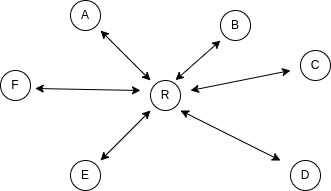
\includegraphics[width=\textwidth]{images/Centralized.png}
    \caption{Cellular network topology}
    \label{fig:centralized}
  \end{subfigure}
  \hfill
  \begin{subfigure}[b]{0.48\textwidth}
    \centering
    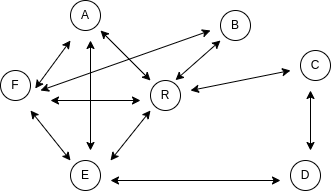
\includegraphics[width=\textwidth]{images/Decentralized.png}
    \caption{Ad-hoc network topology}
    \label{fig:decentralized}
  \end{subfigure}
  \caption{Network topology models for geodistributed agents. Edges represent communication links (bidirectional for simplicity).}
  \label{fig:nettopology}
\end{figure}

One can also imagine hybrid models, such as an ad-hoc arrangement of
localized cells. In general, one expects more centralized topologies to
be simpler for application developers to reason about, but to require
more physical infrastructure and support. On the other hand, the ad-hoc
model is more fault resistant, but more complicated to implement and
potentially offering fewer assurancess about performance. In either
case, higher-level applications such as shared memory abstractions
should be tuned for the networking environment. It would be even better
if this tuning can take place dynamically, with applications
reconfiguring manually or automatically to the particulars of the
operating environment. This requires examining the relationship between
the application and networking layers, rather than treating them as
separate blackboxes.

\hypertarget{delay-tolerant-networking}{%
  \subsection{Delay-tolerant networking}\label{delay-tolerant-networking}}

\hypertarget{ad-hoc-dtns}{%
  \subsection{Ad-hoc DTNs}\label{ad-hoc-dtns}}

An interesting possibility is for the \emph{network} to automatically
configure itself to the quality-of-service needs of the application. For
example, a client that receives a lot of requests may be marked as a
preferred client and given higher-priority access to the network. If UAV
vehicles can be used to route messages by acting as mobile transmission
base stations, one can imagine selecting a flight pattern based on
networking needs. For example, if the communication between two
firefighting teams is obstructed by a geographical feature, a UAV could
be dispatched to provide overhead communication support. Such an
arrangement could greatly blur the line between the networking and
application layers.

\hypertarget{software-defined-networking}{%
  \subsection{Software-defined
    networking}\label{software-defined-networking}}

\hypertarget{verification-of-networking-protocols}{%
  \subsection{Verification of networking
    protocols}\label{verification-of-networking-protocols}}

\newpage

\hypertarget{continuous-consistency}{%
  \section{Continuous Consistency}\label{continuous-consistency}}

\label{sec:continuous-consistency}

Strong consistency is a discrete proposition: an application provides
strong consistency or it does not. For many real-world applications, it
evidently makes sense to work with data that is consistent up to some
\(\epsilon \in \mathbb{R}^{\geq 0}\). Thus, we shift from thinking about
consistency as an all-or-nothing condition, towards consistency as a
bound on inconsistency.

The definition of \(\epsilon\) evidently requires a more or less
application-specific notion of divergence between replicas of a shared
data object. Take, say, an application for disseminating the most
up-to-date visualization of the location of a fire front. It may be
acceptable if this information appears 5 minutes out of date to a
client, but unacceptable if it is 30 minutes out of date. That is, we
could measure consistency with respect to \emph{time}. One should expect
the exact tolerance for \(\epsilon\) will be depend very much on the
client, among other things. For example, firefighters who are very close
to a fire have a lower tolerance for stale information than a central
client keeping only a birds-eye view of several fire fronts
simultaneously.

Now suppose many disaster-response agencies coordinate with to update
and propagate information about the availability of resources. A client
may want to lookup the number of vehicles of a certain type that are
available to be dispatched within a certain geographic range. We may
stipulate that the value read by a client should always be \(4\) of the
actual number, i.e.~we could measure inconsistency with respect to some
numerical value.

In the last example, the reader may wonder we should tolerate a client
to read a value that is incorrect by 4, when clearly it is better to be
incorrect by 0. Intuitively, the practical benefit of tolerating weaker
values is to tolerate a greater level of imperfection in network
communications. For example, suppose Alice and Bob are individually
authorized to dispatch vehicles from a shared pool. In the event that
they cannot share a message.

Or, would could ask that the the value is a conservative estimate,
possibly lower but not higher than the actual amount. In these examples,
we measure inconsistency in terms of a numerical value.

As a third example,

By varying \(\epsilon\), one can imagine consistency as a continuous
spectrum. In light of the CAP theorem, we should likewise expect that
applications with weaker consistency requirements (high \(\epsilon\))
should provide higher availability, all other things being equal.

Yu and Vahdat explored the CAP tradeoff from this perspective in a
series of papers \cite{2000tact 2000tactalgorithms 10.5555/1251229.1251250 DBLP:conf/icdcs/YuV01 2002tact}
propose a theory of \emph{conits}, a logical unit of data subject to
their three metrics for measuring consistency. By controlling the
threshold of acceptable inconsistency of each conit as a continuous
quantity, applications can exercise precise control the tradeoff between
consistency and performance, trading one for the other in a gradual
fashion.

They built a prototype toolkit called TACT, which allows applications to
specify precisely their desired levels of consistency for each conit. An
interesting aspect of this work is that consistency can be tuned
\emph{dynamically}. This is desirable because one does not know a priori
how much consistency or availability is acceptable.

The biggest question one must answer is the competing goals of
generality and practicality. Generality means providing a general notion
of measuring \(\epsilon\), while practicality means enforcing
consistency in a way that can exploit weakened consistency requirements
to offer better overall performance.

\begin{itemize}
\item
  The tradeoff of CAP is a continuous spectrum between linearizability
  and high-availability. More importantly, it can be tuned in real time.
\item
  TACT captures neither CAP-consistency (i.e.~neither atomic nor
  sequential consistency) nor CAP-availability (read and write requests
  may be delayed indefinitely if the system is unable to enforce
  consistency requirements because of network issues).
\end{itemize}

\hypertarget{causal-consistency-1}{%
  \subsection{Causal consistency}\label{causal-consistency-1}}

Causal consistency is that each clients is consistent with a total order
that contains the happened-before relation. It does not put a bound on
divergence between replicas. Violations of causal consistency can
present clients with deeply counterintuitive behavior.

\begin{itemize}
  \tightlist
\item
  In a group messaing application, Alice posts a message and Bob
  replies. On Charlie's device, Bob's reply appears before Alice's
  original message.
\item
  Alice sees a deposit for \$100 made to her bank account and, because
  of this, decides to withdraw \$50. When she refreshes the page, the
  deposit is gone and her account is overdrawn by \(50\). A little while
  later, she refreshes the page and the deposit reappears, but a penalty
  has been assessed for overdrawing her account.
\end{itemize}

In these scenarios, one agent takes an action \emph{in response to} an
event, but other processes observe these causally-related events taking
place in the opposite order. In the first example, Charlie is able to
observe a response to a message he does not see, which does not make
sense to him. In the second example, Alice's observation at one instance
causes her to take an action, but at a later point the cause for her
actions appears to have occurred after her response to it. Both of these
scenarios already violate atomic and sequential consistency because
those models enforce a system-wide total order of events. Happily, they
are also ruled out by causally consistent systems. The advantage of the
causal consistency model is that it rules out this behavior without
sacrificing system availability, as shown below.

Causal consistency enforces a global total order on events that are
\emph{causally related}. Here, causal relationships are estimated very
conservatively: two events are potentially causally if there is some way
that the outcome of one could have influenced another.

\begin{figure}
  \center
  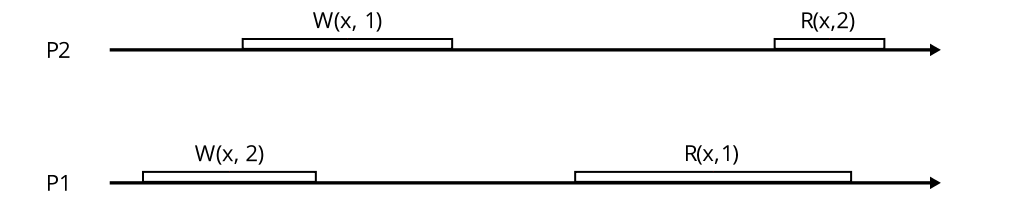
\includegraphics[scale=0.4]{images/causal1.png}
  \caption{A causally consistent, non-sequentially-consistent execution}
\end{figure}

\begin{lemma}
  Sequential consistency implies causal consistency.
\end{lemma}
\begin{proof}
  This is immediate from the definitions. Sequential consistency
  requires all processes to observe the same total order of events,
  where this total order must respect program order. Causal consistency
  only requires processes to agree on events that are potentially
  causally related. Program order is a subset of causal order, so any
  sequential executions also respects causal order.
\end{proof}

However, causal consistency is not nearly as strong as sequential
consistency, as processes do not need to agree on the order of events
with no causal relation between them. This weakness is evident in the
fact that the CAP theorem does not rule out highly available systems
that maintain causal consistency even during network partitions.

\begin{lemma}
  A causally consistent system need not be unavailabile during partitions.
\end{lemma}
\begin{proof}

  Suppose $P_1$ and $P_2$ maintain replicas of a key-value store, as
  before, and suppose they are separated by a partition. The strategy is
  simple: each process immediately handles read requests by reading from
  its local replica, and handles write requests by applying the update
  to its local replica. It is easy to see this leads to causally
  consistent histories. Intuitively, the fact that no information flows
  between the processes also means the events of each process are not
  related by causality, so causality is not violated.  \end{proof}

Note that in this scenario, a client's requests are always routed to the
same processor. If a client's requests can be routed to any node, causal
consistency cannot be maintained without losing availability. One
sometimes says that causal consistency is ``sticky available'' because
clients must stick to the same processor during partitions.

The fact that causal consistency can be maintained during partitions
suggests it is too weak. Indeed, there are no guarantees about the
difference in values for \(x\) and \(y\) across the two replicas.

\hypertarget{tact-system-model}{%
  \subsection{TACT system model}\label{tact-system-model}}

As in Section \ref{sec:background}, we assume a distributed set of
processes collaborate to maintain local replicas of a shared data object
such as a database. Processes accept read and write requests from
clients to update items, and they communicate with each other to ensure
to ensure that all replicas remain consistent.

However, access to the data store is mediated by a middleware library,
which sits between the local copy of the replica and the client. At a
high level, TACT will allow an operation to take place if it does not
violate user-specific consistency bounds. If allowing an operation to
proceed would violate consistency constraints, the operation blocks
until TACT synchronizes with one or more other remote replicas. The
operation remains blocked until TACT ensures that executing it would not
violate consistency requirements.

\[\textrm{Consistency} = \langle \textrm{Numerical error, \textrm{Order error}, \textrm{Staleness}} \rangle.\]

Processes forward accesses to TACT, which handles commiting them to the
store. TACT may not immediately process the request---instead it may
need to coordinate with other processes to enforce consistency. When
write requests are processed (i.e.~when a response is sent to the
originating client), they are only commited in a \emph{tenative} state.
Tentative writes eventually become fully committed at some point in the
future, but when they are commited, they may be reordered. After
fullying committing, writes are in a total order known to all processes.

\begin{figure}[h]
  \center
  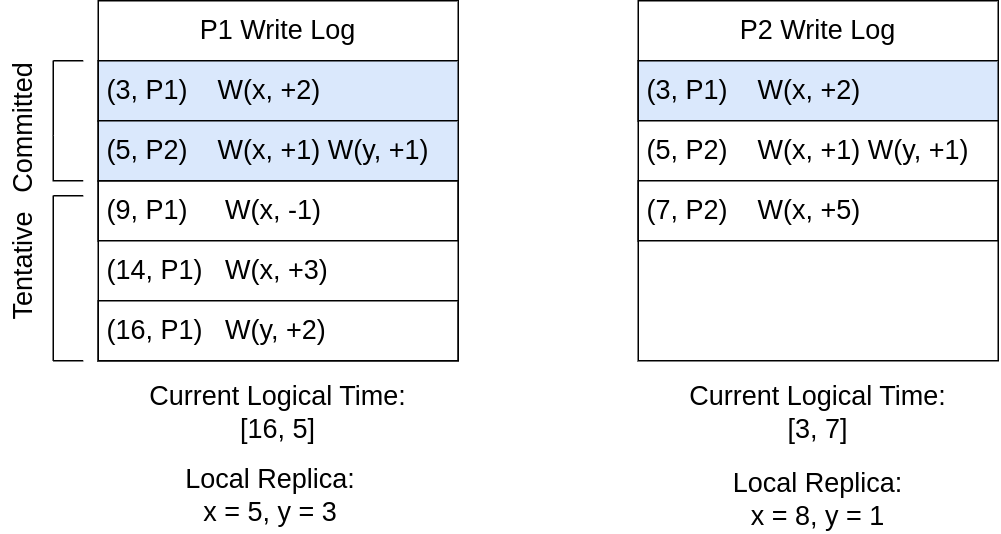
\includegraphics[scale=0.4]{images/TACT Logs.png}
  \caption{Snapshot of two local replicas using TACT}
  \label{fig:tact_logs}
\end{figure}

A write access \(W\) can separately quantify its \emph{numerical weight}
and \emph{order weight} on conit \(F\). Application programmers have
multiple forms of control:

Consistency is enforced by the application by setting bounds on the
consistency of read accesses. The TACT framework then enforces these
consistency levels.

\hypertarget{measuring-consistency-on-conits}{%
  \subsection{Measuring consistency on
    conits}\label{measuring-consistency-on-conits}}

\hypertarget{numerical-consistency}{%
  \paragraph{Numerical consistency}\label{numerical-consistency}}

\hypertarget{order-consistency}{%
  \paragraph{Order consistency}\label{order-consistency}}

When the number of tentative (uncommitted) writes is high, TACT executes
a write commitment algorithm. This is a \emph{pull-based} approach which
pulls information from other processes in order to advance \(P_i\)'s
vector clock, raising the watermark and hence allowing \(P_i\) to commit
some of its writes.

\hypertarget{real-time-consistency}{%
  \paragraph{Real time consistency}\label{real-time-consistency}}

\hypertarget{enforcing-inconsistency-bounds}{%
  \subsection{Enforcing inconsistency
    bounds}\label{enforcing-inconsistency-bounds}}

\hypertarget{numerical-consistency-1}{%
  \paragraph{Numerical consistency}\label{numerical-consistency-1}}

We describe split-weight AE. Yu and Vahdat also describe two other
schemes for bounding numerical error. One, compound AE, bounds absolute
error trading space for communication overhead. In their simulations,
they found minimal benefits to this tradeoff in general. It is possible
that for specific applications the savings are worth it. They also
consider a scheme, Relative NE, which bounds the relative error.

\hypertarget{order-consistency-1}{%
  \paragraph{Order consistency}\label{order-consistency-1}}

\hypertarget{real-time-consistency-1}{%
  \paragraph{Real time consistency}\label{real-time-consistency-1}}

\hypertarget{future-work}{%
  \subsection{Future work}\label{future-work}}

\hypertarget{data-fusion}{%
  \section{Data Fusion}\label{data-fusion}}

\cite{1999:lucien-datafusion}

\label{sec:data-fusion}

Strong consistency models provide the abstraction of an idealized global
truth. In the case of conits, the numerical, commit-order, and real-time
errors are measured with respect to an idealized global state of the
database. This state may not exist on any one replica, but it is the
state each replica would converge to if it were to see all remaining
unseen updates.

We consider distributed applications that receive data from many
different sources, such as from a sensor network (broadly defined). It
will often be the case that some sources of data should be expected to
agree with each other, but they may not. A typical scenario, we want to
integrate these data into a larger model of some kind. Essentially take
a poll, and attempt to synthesize a global picture that agrees as much
as possible with the data reported from the sensor network.

Here, we need a consistency model to measure how successful our attempts
are to synthesize a global image. And to tell us how much our sensors
agree. Ideally, we could use this system to diagnose disagreements
between sensors, identifying sensors that appear to be malfunctioning,
or to detect abberations that necessitate a response.

\hypertarget{fusion-centers}{%
  \subsection{Fusion centers}\label{fusion-centers}}

To be written.

\hypertarget{sheaf-theory}{%
  \subsection{Sheaf theory}\label{sheaf-theory}}

\hypertarget{introduction-to-presheaves}{%
  \subsubsection{Introduction to
    presheaves}\label{introduction-to-presheaves}}

\begin{definition}
  A \emph{partially order-indexed family of sets} is a family of sets indexed by a partially-ordered set,
  such that orders between the indices correspond to functions between the sets.
\end{definition}

We can also set \((P, \leq)\) \emph{acts on} the set
\(\{S_i\}_{i \in I}\).

\begin{definition}
  A \emph{semiautomaton} is a monoid paired with a set.
\end{definition}

This is also called a \emph{monoid action} on the set.

\begin{definition}
  A copresheaf is a *category acting on a family of sets*.
\end{definition}

\begin{definition}
  A presheaf is a *category acting covariantly on a family of sets*.
\end{definition}

\hypertarget{introduction-to-sheaves}{%
  \subsubsection{Introduction to sheaves}\label{introduction-to-sheaves}}

To be written.

\hypertarget{the-consistency-radius}{%
  \subsubsection{The consistency radius}\label{the-consistency-radius}}

To be written.

\hypertarget{conclusion}{%
  \section{Conclusion}\label{conclusion}}

\label{sec:conclusion}

To be written.

\section*{Bibliography}\label{bibliography}
\addcontentsline{toc}{section}{Bibliography}

\bibliographystyle{abbrv}
\bibliography{bibliography}

\end{document}
